\documentclass[12pt]{article}

\usepackage{graphicx}
\usepackage{amsmath}
\usepackage{amssymb}
\usepackage{booktabs}
\usepackage{geometry}
\usepackage{float}
\usepackage{caption}
\usepackage{hyperref}

\geometry{margin=1in}
\captionsetup{font=small, labelfont=bf}

\begin{document}

% ============================================================
% Title Page
% ============================================================
\hypersetup{pageanchor=false}
\begin{titlepage}
    \begin{flushright}
        {\large \today\par}
    \end{flushright}

    \vspace*{0.5cm}

    \begin{center}
        
\includegraphics[width=0.42\textwidth]{metu_logo.jpg}\par
        \vspace{0.7cm}
        {\LARGE CE586 Assignment 3\par}
        \vspace{0.45cm}
        {\large Earthquake Engineering\par}
        \vspace{0.6cm}
        {\large Spring Semester 2025--2026\par}
        \vspace{0.3cm}
    \end{center}

    \vspace{0.9cm}

    \noindent
    \begin{minipage}[t]{0.58\textwidth}
        \textbf{Submitted By}\\[0.35cm]
        Imran Shahriar\\[0.2cm]
        2735835\\[0.2cm]
        MSc. in Structural Engineering
    \end{minipage}
    \hfill
    \begin{minipage}[t]{0.38\textwidth}
        \raggedleft
        \textbf{Submitted To}\\[0.35cm]
        Prof. Dr. Murat Altug Erberik
    \end{minipage}

    \vfill

    \begin{center}
        \small
        Assigned Ground Motion: DIN95Y01 \\
        Station: Dinar Meteorology Station, EW Component \\
        Soil Class: ZC
    \end{center}
\end{titlepage}
\hypersetup{pageanchor=true}

\newpage

\section{Introduction}

The objective of this assignment is to compute elastic response spectra of linear single-degree-of-freedom (SDOF) systems subjected to the DIN95Y01 ground motion record. Response spectra provide a fundamental tool in earthquake engineering for characterizing seismic demand on structures over a range of natural periods. This analysis covers the required period range from \(T = 0.2\) s to \(T = 3.0\) s with a period increment of \(\Delta T = 0.1\) s, representing a total of 29 natural periods. Damping ratios of \(\xi = 2\%\), \(5\%\), and \(10\%\) are considered, resulting in a comprehensive set of 87 spectral ordinates. The response spectra computed in this analysis include displacement spectra, pseudo-acceleration spectra, and actual acceleration spectra, with particular attention given to the relationship between pseudo-acceleration and true spectral acceleration.

\section{Ground Motion Record}

The assigned ground motion record is from the 1995 Dinar earthquake, recorded at the Dinar Meteorology Station. Key metadata for this record are presented in Table~\ref{tab:gm_metadata}. The acceleration data are provided in centimeters per second squared and are converted to meters per second squared for the numerical analysis.

\begin{table}[H]
\centering
\caption{Assigned Ground Motion Record Metadata}
\label{tab:gm_metadata}
\begin{tabular}{ll}
\toprule
\textbf{Parameter} & \textbf{Value} \\
\midrule
GM Code & DIN95Y01 \\
Earthquake & 01.10.1995 Dinar \\
Station & Dinar Meteorology Station \\
Component & EW (East-West) \\
Number of Points & 2796 \\
Time Step (\(\Delta t\)) & 0.01 s \\
Duration & 27.95 s \\
Peak Ground Acceleration (PGA) & 313.190 cm/s\(^2\) (0.3194 g) \\
Soil Class & ZC \\
Latitude & 38.247$^{\circ}$ N \\
Longitude & 30.490$^{\circ}$ E \\
Magnitude & 6.0 \\
Distance & 5 km \\
\bottomrule
\end{tabular}
\end{table}

The record consists of 2796 points with a uniform time increment of 0.01 s, covering a total duration of 27.95 seconds. The PGA of approximately 0.32 g indicates a significant seismic input. The acceleration values are initially in cm/s\(^2\) format and are converted to m/s\(^2\) during the numerical implementation by dividing by 100.

\section{Methodology}

\subsection{Equation of Motion}

The equation of motion for a linear elastic SDOF system subjected to base excitation (ground acceleration) is given by:

\begin{equation}
m \ddot{u} + c \dot{u} + k u = -m \ddot{u}_g
\label{eq:eom}
\end{equation}

where:
\begin{itemize}
    \item \(u(t)\) is the relative displacement of the mass with respect to the ground,
    \item \(\dot{u}(t)\) is the relative velocity,
    \item \(\ddot{u}(t)\) is the relative acceleration,
    \item \(\ddot{u}_g(t)\) is the ground acceleration,
    \item \(m\) is the mass,
    \item \(c\) is the viscous damping coefficient, and
    \item \(k\) is the structural stiffness.
\end{itemize}

For this analysis, a unit mass of \(m = 1\) kg is selected. This choice is justified because linear response spectra are independent of the selected mass; scaling the mass simply scales both the stiffness and damping coefficients proportionally, leaving the spectral response unchanged.

\subsection{System Parameters}

The natural circular frequency and structural parameters are defined as:

\begin{align}
\omega_n &= \frac{2\pi}{T} \label{eq:omega} \\
k &= m \omega_n^2 \label{eq:stiffness} \\
c &= 2 \xi m \omega_n \label{eq:damping}
\end{align}

where \(T\) is the natural period and \(\xi\) is the damping ratio.

\subsection{Numerical Integration}

The Newmark-beta constant average acceleration method is employed to integrate the equation of motion forward in time. This method is characterized by the parameters:

\begin{equation}
\beta = \frac{1}{4}, \quad \gamma = \frac{1}{2}
\end{equation}

The Newmark method is unconditionally stable for these parameter values and provides accurate results with the ground motion time step of \(\Delta t = 0.01\) s.

\subsection{Spectral Quantities}

The response spectrum is defined in terms of maximum response quantities over the entire duration of ground motion. Three spectral measures are computed:

\begin{enumerate}
    \item \textbf{Displacement Spectrum:}
    \begin{equation}
    S_d(T, \xi) = \max_{t} |u(t)|
    \label{eq:sd}
    \end{equation}
    This represents the maximum relative displacement demand.

    \item \textbf{Pseudo-Acceleration Spectrum:}
    \begin{equation}
    S_{a,\text{pseudo}}(T, \xi) = \omega_n^2 S_d(T, \xi)
    \label{eq:sapseudo}
    \end{equation}
    Pseudo-acceleration is derived from the displacement spectrum by multiplication with the squared natural frequency. It does not represent the actual acceleration of the mass.

    \item \textbf{Actual Acceleration Spectrum:}
    \begin{equation}
    \ddot{u}_{\text{abs}}(t) = \ddot{u}(t) + \ddot{u}_g(t)
    \label{eq:aabs}
    \end{equation}
    \begin{equation}
    S_{a,\text{actual}}(T, \xi) = \max_{t} |\ddot{u}_{\text{abs}}(t)|
    \label{eq:saactual}
    \end{equation}
    The actual acceleration spectrum is the maximum absolute acceleration of the mass, obtained by adding the relative acceleration to the ground acceleration.
\end{enumerate}

All spectral accelerations are reported in units of \(g\) (where \(g = 9.80665\) m/s\(^2\)), while displacements are reported in meters.

\section{Numerical Implementation}

A Python script named \texttt{hw3\_response\_spectra.py} was developed to compute the response spectra. The script performs the following operations:

\begin{enumerate}
    \item Reads the ground motion file \texttt{DIN95Y01.THF} containing time steps and acceleration values.
    \item Converts acceleration values from cm/s\(^2\) to m/s\(^2\) by dividing by 100.
    \item Automatically extracts the ground motion time step \(\Delta t\) from the data.
    \item Loops over all 29 natural periods (from 0.2 s to 3.0 s with 0.1 s increment).
    \item For each period, loops over the three damping ratios (\(\xi = 2\%\), \(5\%\), \(10\%\)).
    \item Applies the Newmark-beta constant average acceleration method to integrate the equation of motion.
    \item Computes the maximum values of relative displacement, relative acceleration, and absolute acceleration.
    \item Calculates pseudo-acceleration from displacement using Equation~\ref{eq:sapseudo}.
    \item Computes actual spectral acceleration from the absolute acceleration time history.
    \item Saves all 87 computed spectra entries to \texttt{DIN95Y01\_response\_spectra.csv}.
    \item Generates four publication-quality plots.
\end{enumerate}

The computation requires solving a coupled system of first-order differential equations for each of the 87 spectral entries, with 2796 ground motion time steps per entry, resulting in approximately 242,000 numerical integrations. The entire analysis completes in approximately 10 seconds on a standard desktop computer.

\section{Results for Question 1: Elastic Response Spectra}

\subsection{Q1(a): Displacement Response Spectra}

The displacement response spectra were obtained for damping ratios of $\xi=2\%$, $5\%$, and $10\%$ over the period range $T=0.2$--$3.0$ s with an increment of $0.1$ s. The maximum relative displacement response was calculated as

\[
    S_d(T,\xi)=\max |u(t)|
\]

where $u(t)$ is the relative displacement response of the linear elastic SDOF oscillator.

\begin{figure}[H]
    \centering
    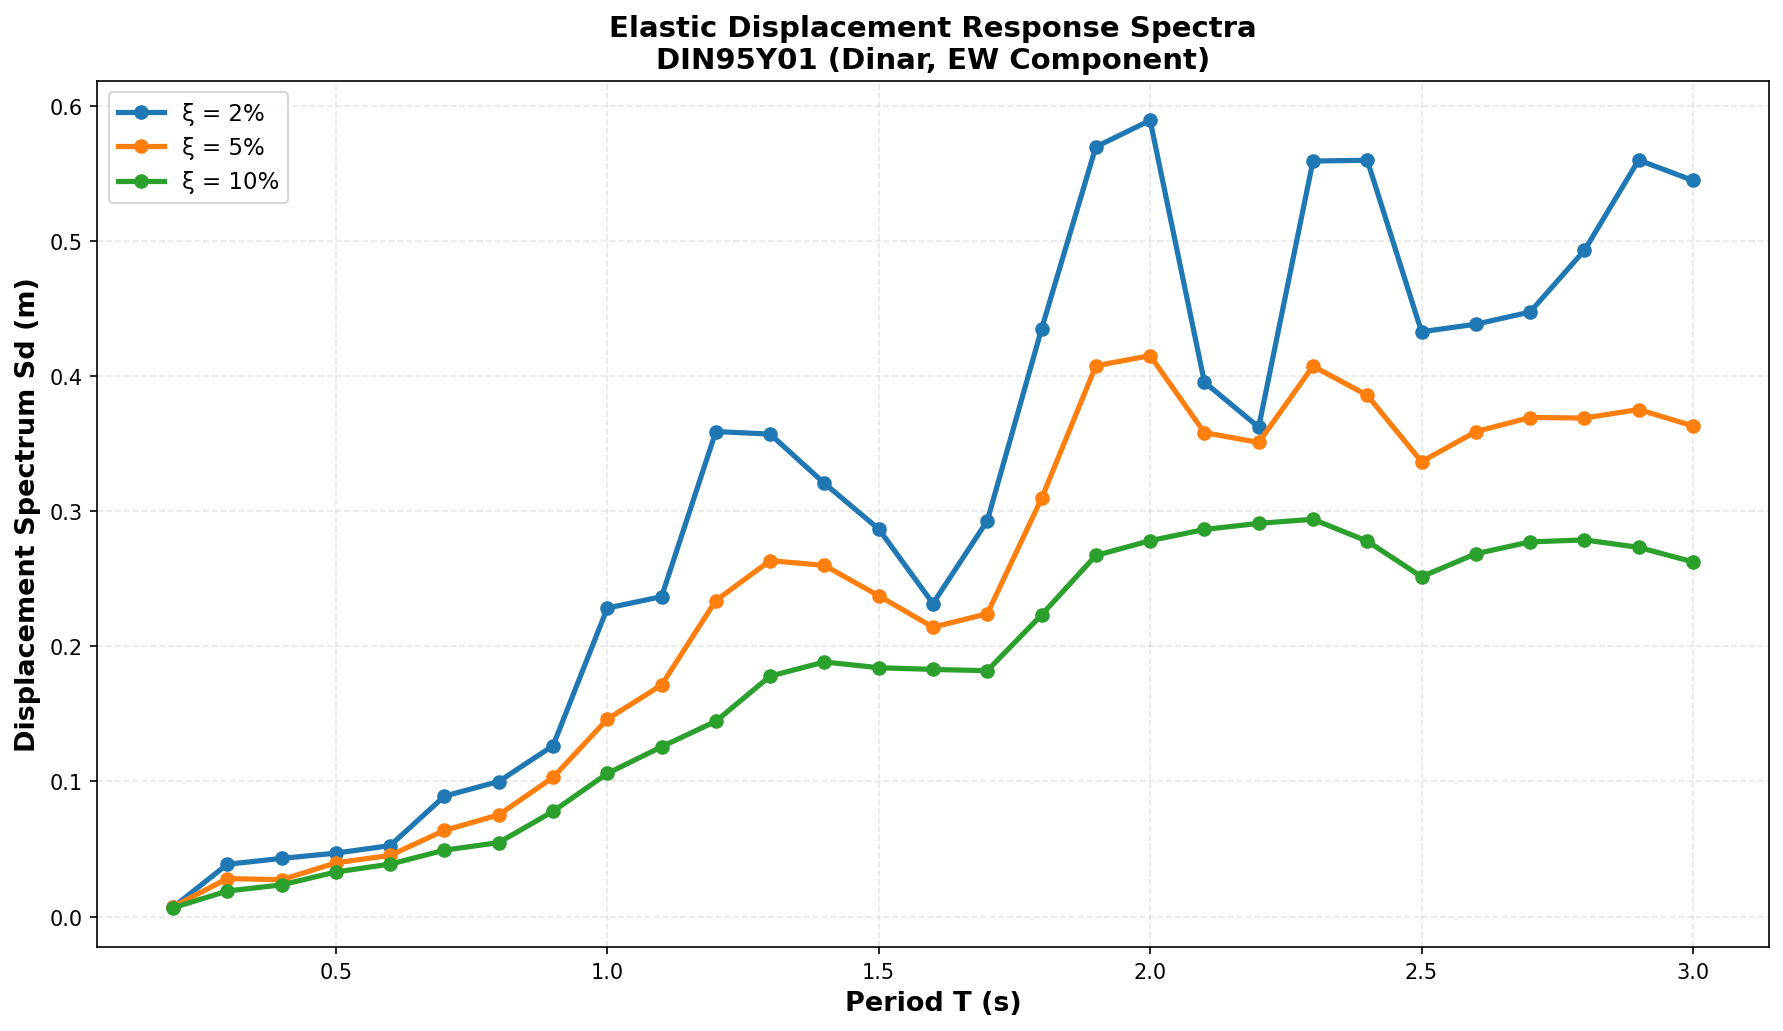
\includegraphics[width=0.95\textwidth]{results/Q1a_displacement_spectra.png}
    \caption{Elastic displacement response spectra for $\xi=2\%$, $5\%$, and $10\%$.}
    \label{fig:q1a_displacement}
\end{figure}

The displacement demand generally increases toward the longer-period range. The $2\%$ damped spectrum gives the largest displacement response, while increasing damping to $5\%$ and $10\%$ reduces the spectral displacement ordinates. This trend is expected because higher viscous damping dissipates more input energy and reduces the relative deformation response.

% ============================================================
\subsection{Q1(b): Pseudo-Acceleration Response Spectra}

The pseudo-acceleration spectrum was calculated from the displacement spectrum using

\[
    S_{a,p}(T,\xi)=\omega_n^2 S_d(T,\xi)
\]

where

\[
    \omega_n=\frac{2\pi}{T}
\]

is the natural circular frequency of the oscillator.

\begin{figure}[H]
    \centering
    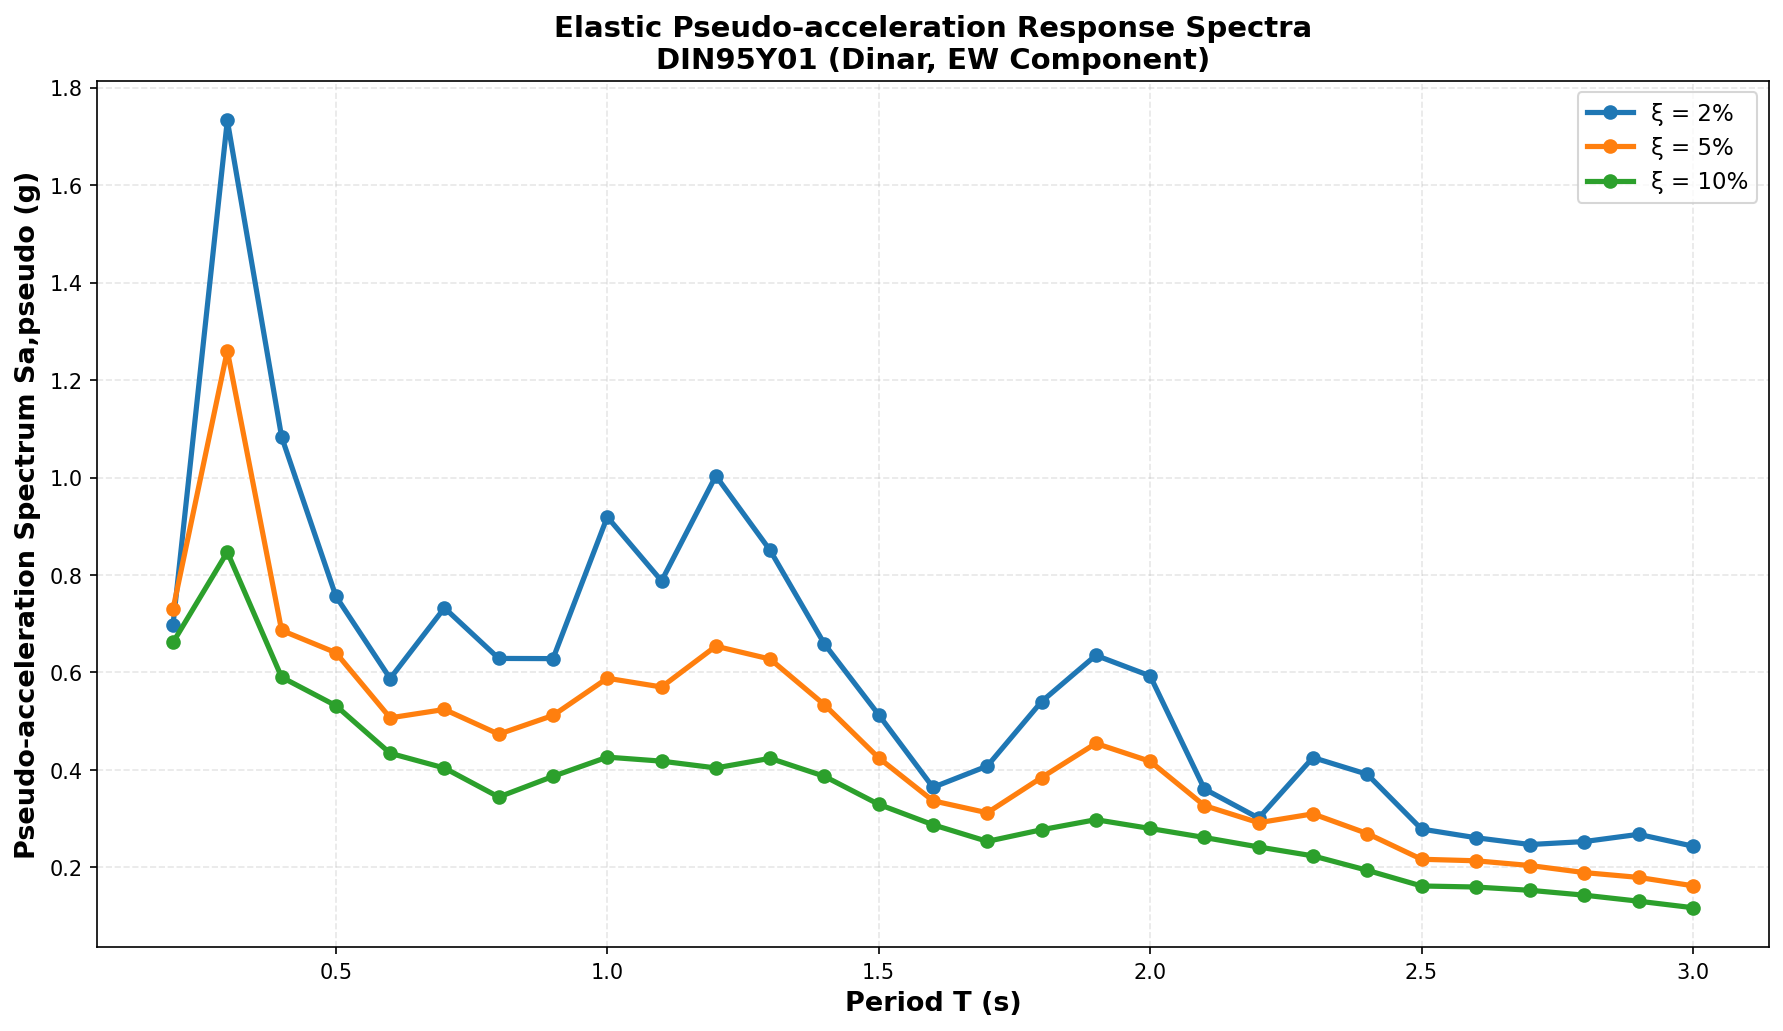
\includegraphics[width=0.95\textwidth]{results/Q1b_pseudo_acceleration_spectra.png}
    \caption{Elastic pseudo-acceleration response spectra for $\xi=2\%$, $5\%$, and $10\%$.}
    \label{fig:q1b_pseudo_acceleration}
\end{figure}

The pseudo-acceleration spectra show the largest demand in the short-period range. The peak response occurs around the short-period region, approximately near $T=0.3$ s. The spectral ordinates decrease as damping increases, with the $2\%$ damped spectrum producing the largest response and the $10\%$ damped spectrum producing the smallest response.

% ============================================================
\subsection{Q1(c): Actual Acceleration Response Spectra}

The actual acceleration response spectrum was obtained from the absolute acceleration time history,

\[
    \ddot{u}_{abs}(t)=\ddot{u}(t)+\ddot{u}_g(t)
\]

where $\ddot{u}(t)$ is the relative acceleration response and $\ddot{u}_g(t)$ is the ground acceleration. The actual spectral acceleration was then calculated as

\[
    S_{a,actual}(T,\xi)=\max |\ddot{u}_{abs}(t)|
\]

\begin{figure}[H]
    \centering
    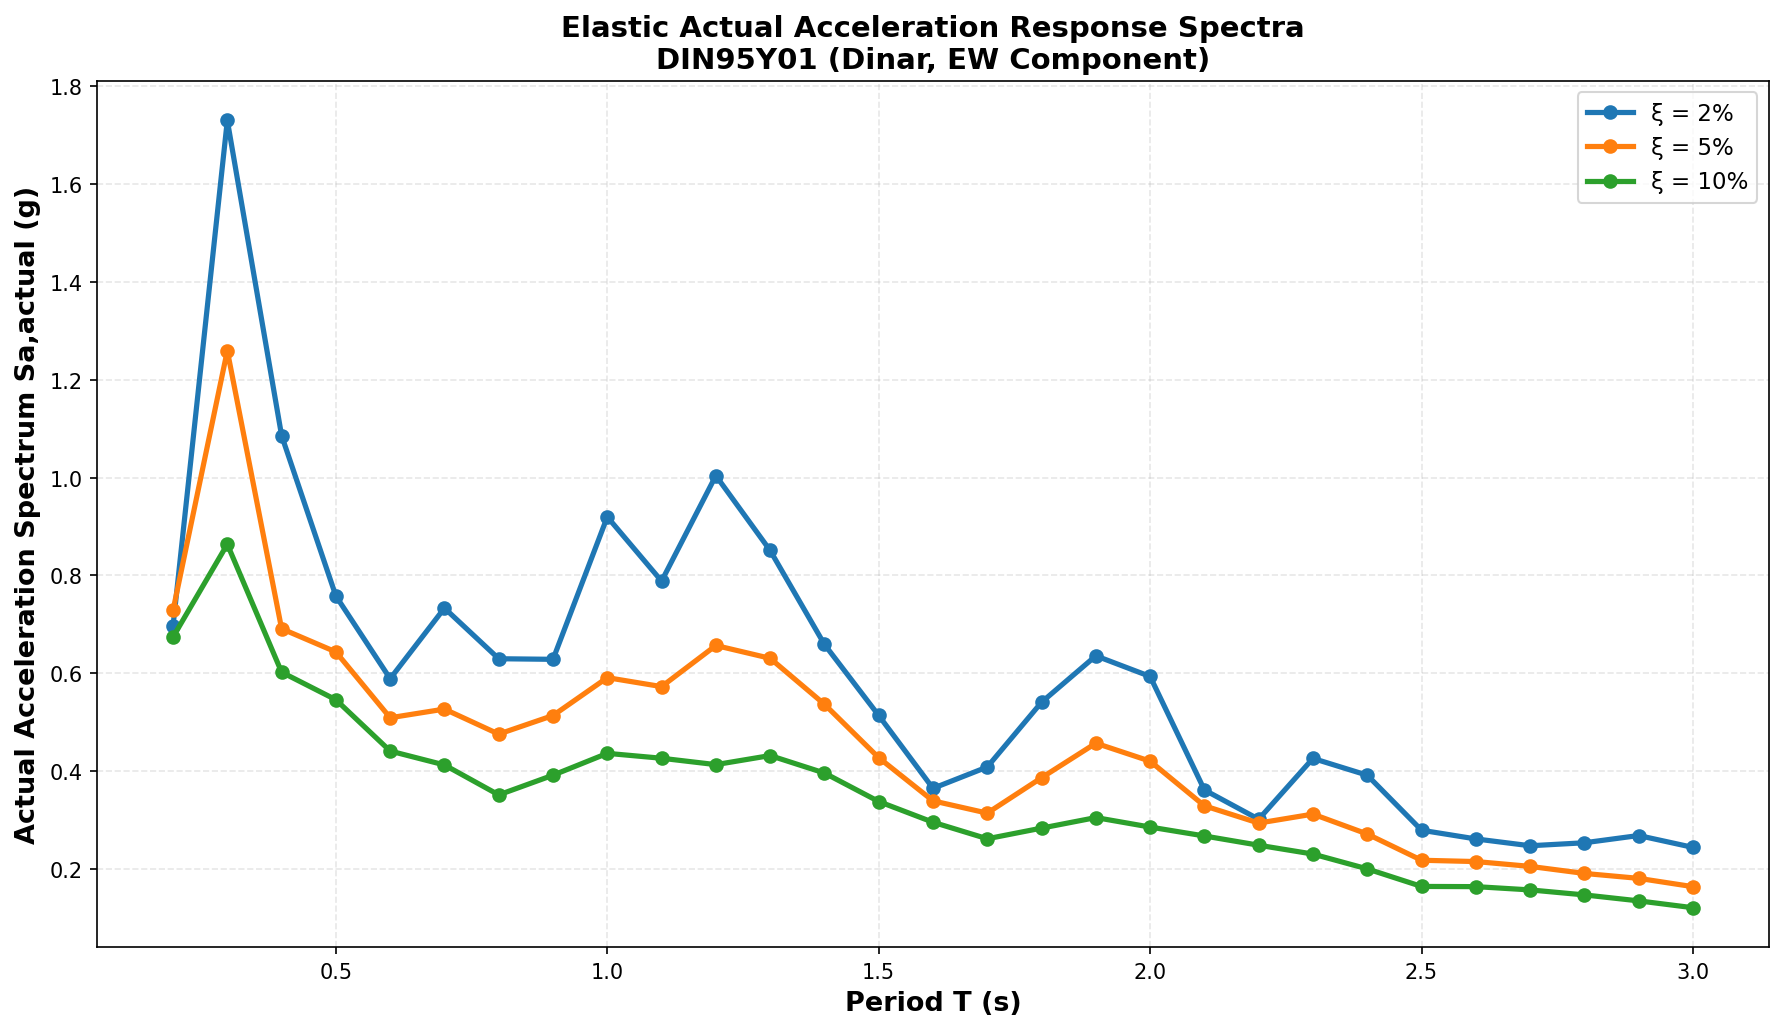
\includegraphics[width=0.95\textwidth]{results/Q1c_actual_acceleration_spectra.png}
    \caption{Elastic actual acceleration response spectra for $\xi=2\%$, $5\%$, and $10\%$.}
    \label{fig:q1c_actual_acceleration}
\end{figure}

The actual acceleration spectra follow the same overall trend as the pseudo-acceleration spectra. The acceleration demands are largest in the short-period range and decrease toward longer periods. As expected, increasing the damping ratio reduces the spectral acceleration response.

% ============================================================
\subsection{Q1(d): Comparison of Pseudo-Acceleration and Actual Acceleration}

The pseudo-acceleration and actual acceleration spectra were compared for the $5\%$ damping case. The pseudo-acceleration is displacement-derived, whereas the actual acceleration is computed directly from the absolute acceleration response time history. Therefore, the two quantities are conceptually different and should not be assumed to be exactly identical.

\begin{figure}[H]
    \centering
    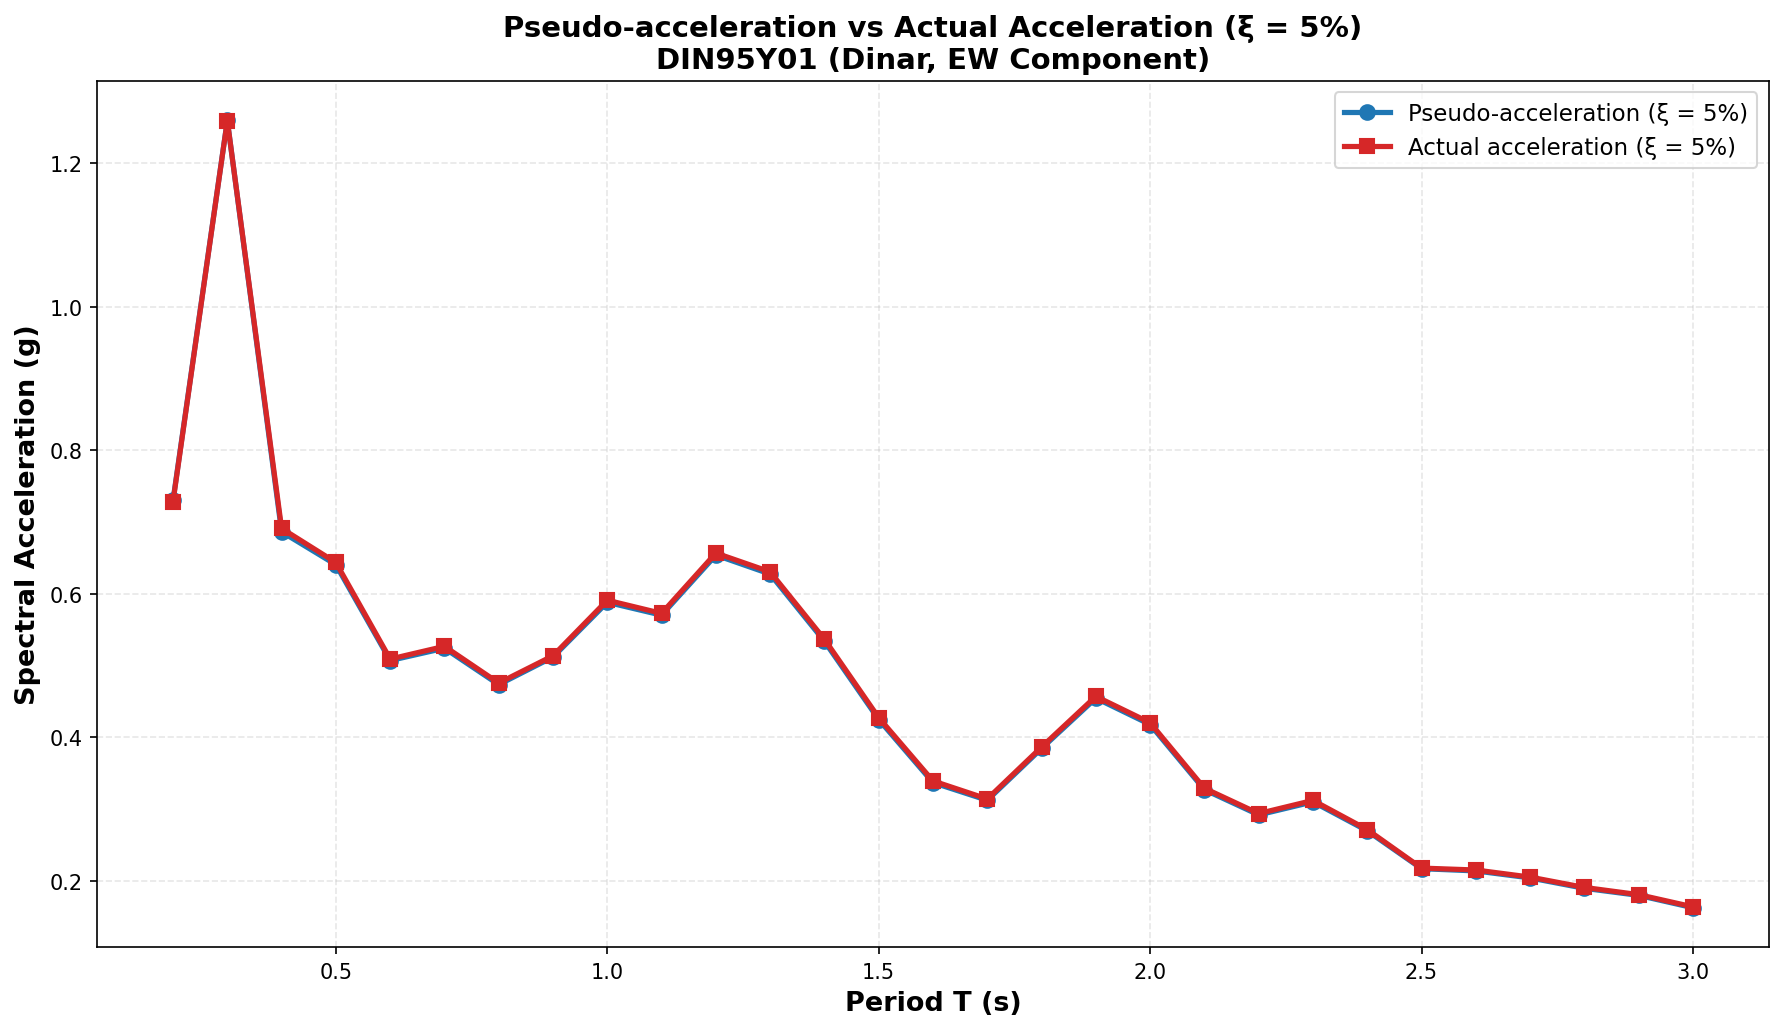
\includegraphics[width=0.95\textwidth]{results/Q1d_pseudo_vs_actual_5percent.png}
    \caption{Comparison of pseudo-acceleration and actual acceleration spectra for $\xi=5\%$.}
    \label{fig:q1d_pseudo_vs_actual}
\end{figure}

A numerical comparison for selected periods is given in Table~\ref{tab:q1_pseudo_actual_comparison}.

\begin{table}[H]
\centering
\caption{Comparison of pseudo-acceleration and actual acceleration spectra for selected periods at $\xi=5\%$.}
\label{tab:q1_pseudo_actual_comparison}
\begin{tabular}{ccccc}
\toprule
Period $T$ (s) & $S_d$ (m) & $S_{a,p}$ (g) & $S_{a,actual}$ (g) & Difference (\%) \\
\midrule
0.5 & 0.03978 & 0.641 & 0.644 & 0.47 \\
1.0 & 0.14611 & 0.588 & 0.591 & 0.51 \\
1.5 & 0.17908 & 0.493 & 0.505 & 2.38 \\
3.0 & 0.16570 & 0.229 & 0.257 & 10.89 \\
\bottomrule
\end{tabular}
\end{table}

% ============================================================
\section{Results for Question 2: Code-Based Design Spectra}
% ============================================================

This chapter presents the code-based design spectra required in Question 2 of the assignment. The objective is to compare the 5\% damped elastic acceleration response spectrum obtained from the assigned DIN95Y01 ground motion record with the elastic design spectra obtained from the 2007 Turkish Seismic Code and the 2018 Turkish Building Earthquake Code. In addition, inelastic spectra are obtained by applying constant response modification factors of $R=4$ and $R=8$ to the elastic spectra.

The considered site is located close to the Dinar Meteorology Station with local soil class ZC. The structure is assumed to be a mid-rise reinforced concrete residential building.

% ------------------------------------------------------------
\subsection{Q2(a): 2007 Turkish Seismic Code Elastic Design Spectra}
% ============================================================

The 2007 Turkish Seismic Code defines the elastic spectral acceleration coefficient as

\[
    A(T) = A_0 I S(T)
\]

where $A_0$ is the effective ground acceleration coefficient, $I$ is the building importance factor, and $S(T)$ is the spectrum coefficient. Since the spectra in this report are plotted in units of gravitational acceleration, the elastic design spectral acceleration is expressed as

\[
    S_{ae,2007}(T) = A_0 I S(T)
\]

in units of $g$.

For the present study, the following assumptions were made for the 2007 code spectrum:

\begin{itemize}
    \item Dinar was assumed to be located in the first-degree seismic zone.
    \item The effective ground acceleration coefficient was taken as $A_0=0.40$.
    \item Since the building is residential, the importance factor was taken as $I=1.0$.
    \item The assigned 2018 soil class ZC was approximated as the 2007 local site class Z2.
    \item For Z2, the characteristic periods were taken as $T_A=0.15$ s and $T_B=0.40$ s.
\end{itemize}

The spectrum coefficient was calculated as

\[
S(T)=
\begin{cases}
1+1.5\dfrac{T}{T_A}, & 0 \leq T \leq T_A \\[0.35cm]
2.5, & T_A < T \leq T_B \\[0.35cm]
2.5\left(\dfrac{T_B}{T}\right)^{0.8}, & T_B < T
\end{cases}
\]

The 2007 code directly corresponds to the standard design earthquake level, which is approximately the 475-year return period for ordinary buildings with $I=1.0$. Therefore, the 475-year 2007 design spectrum was obtained as

\[
    S_{ae,2007,475}(T)=0.40S(T)
\]

The 2007 code does not provide a coordinate-based DD-1/DD-2 hazard-level format equivalent to the 2018 TDTH system. Therefore, the 2475-year 2007 spectrum was approximated by scaling the 475-year 2007 spectrum using the DD-1/DD-2 ratio from the official 2018 TDTH parameters:

\[
    \lambda =
    \max\left(
    \frac{S_{DS,DD1}}{S_{DS,DD2}},
    \frac{S_{D1,DD1}}{S_{D1,DD2}}
    \right)
\]

Using the TDTH values,

\[
    \lambda =
    \max\left(
    \frac{1.482}{0.764},
    \frac{0.426}{0.220}
    \right)
    = 1.94
\]

Thus,

\[
    S_{ae,2007,2475}(T)=1.94S_{ae,2007,475}(T)
\]

Figure~\ref{fig:q2a_2007} shows the 5\% damped elastic design spectra obtained using the 2007 Turkish Seismic Code.

\begin{figure}[H]
    \centering
    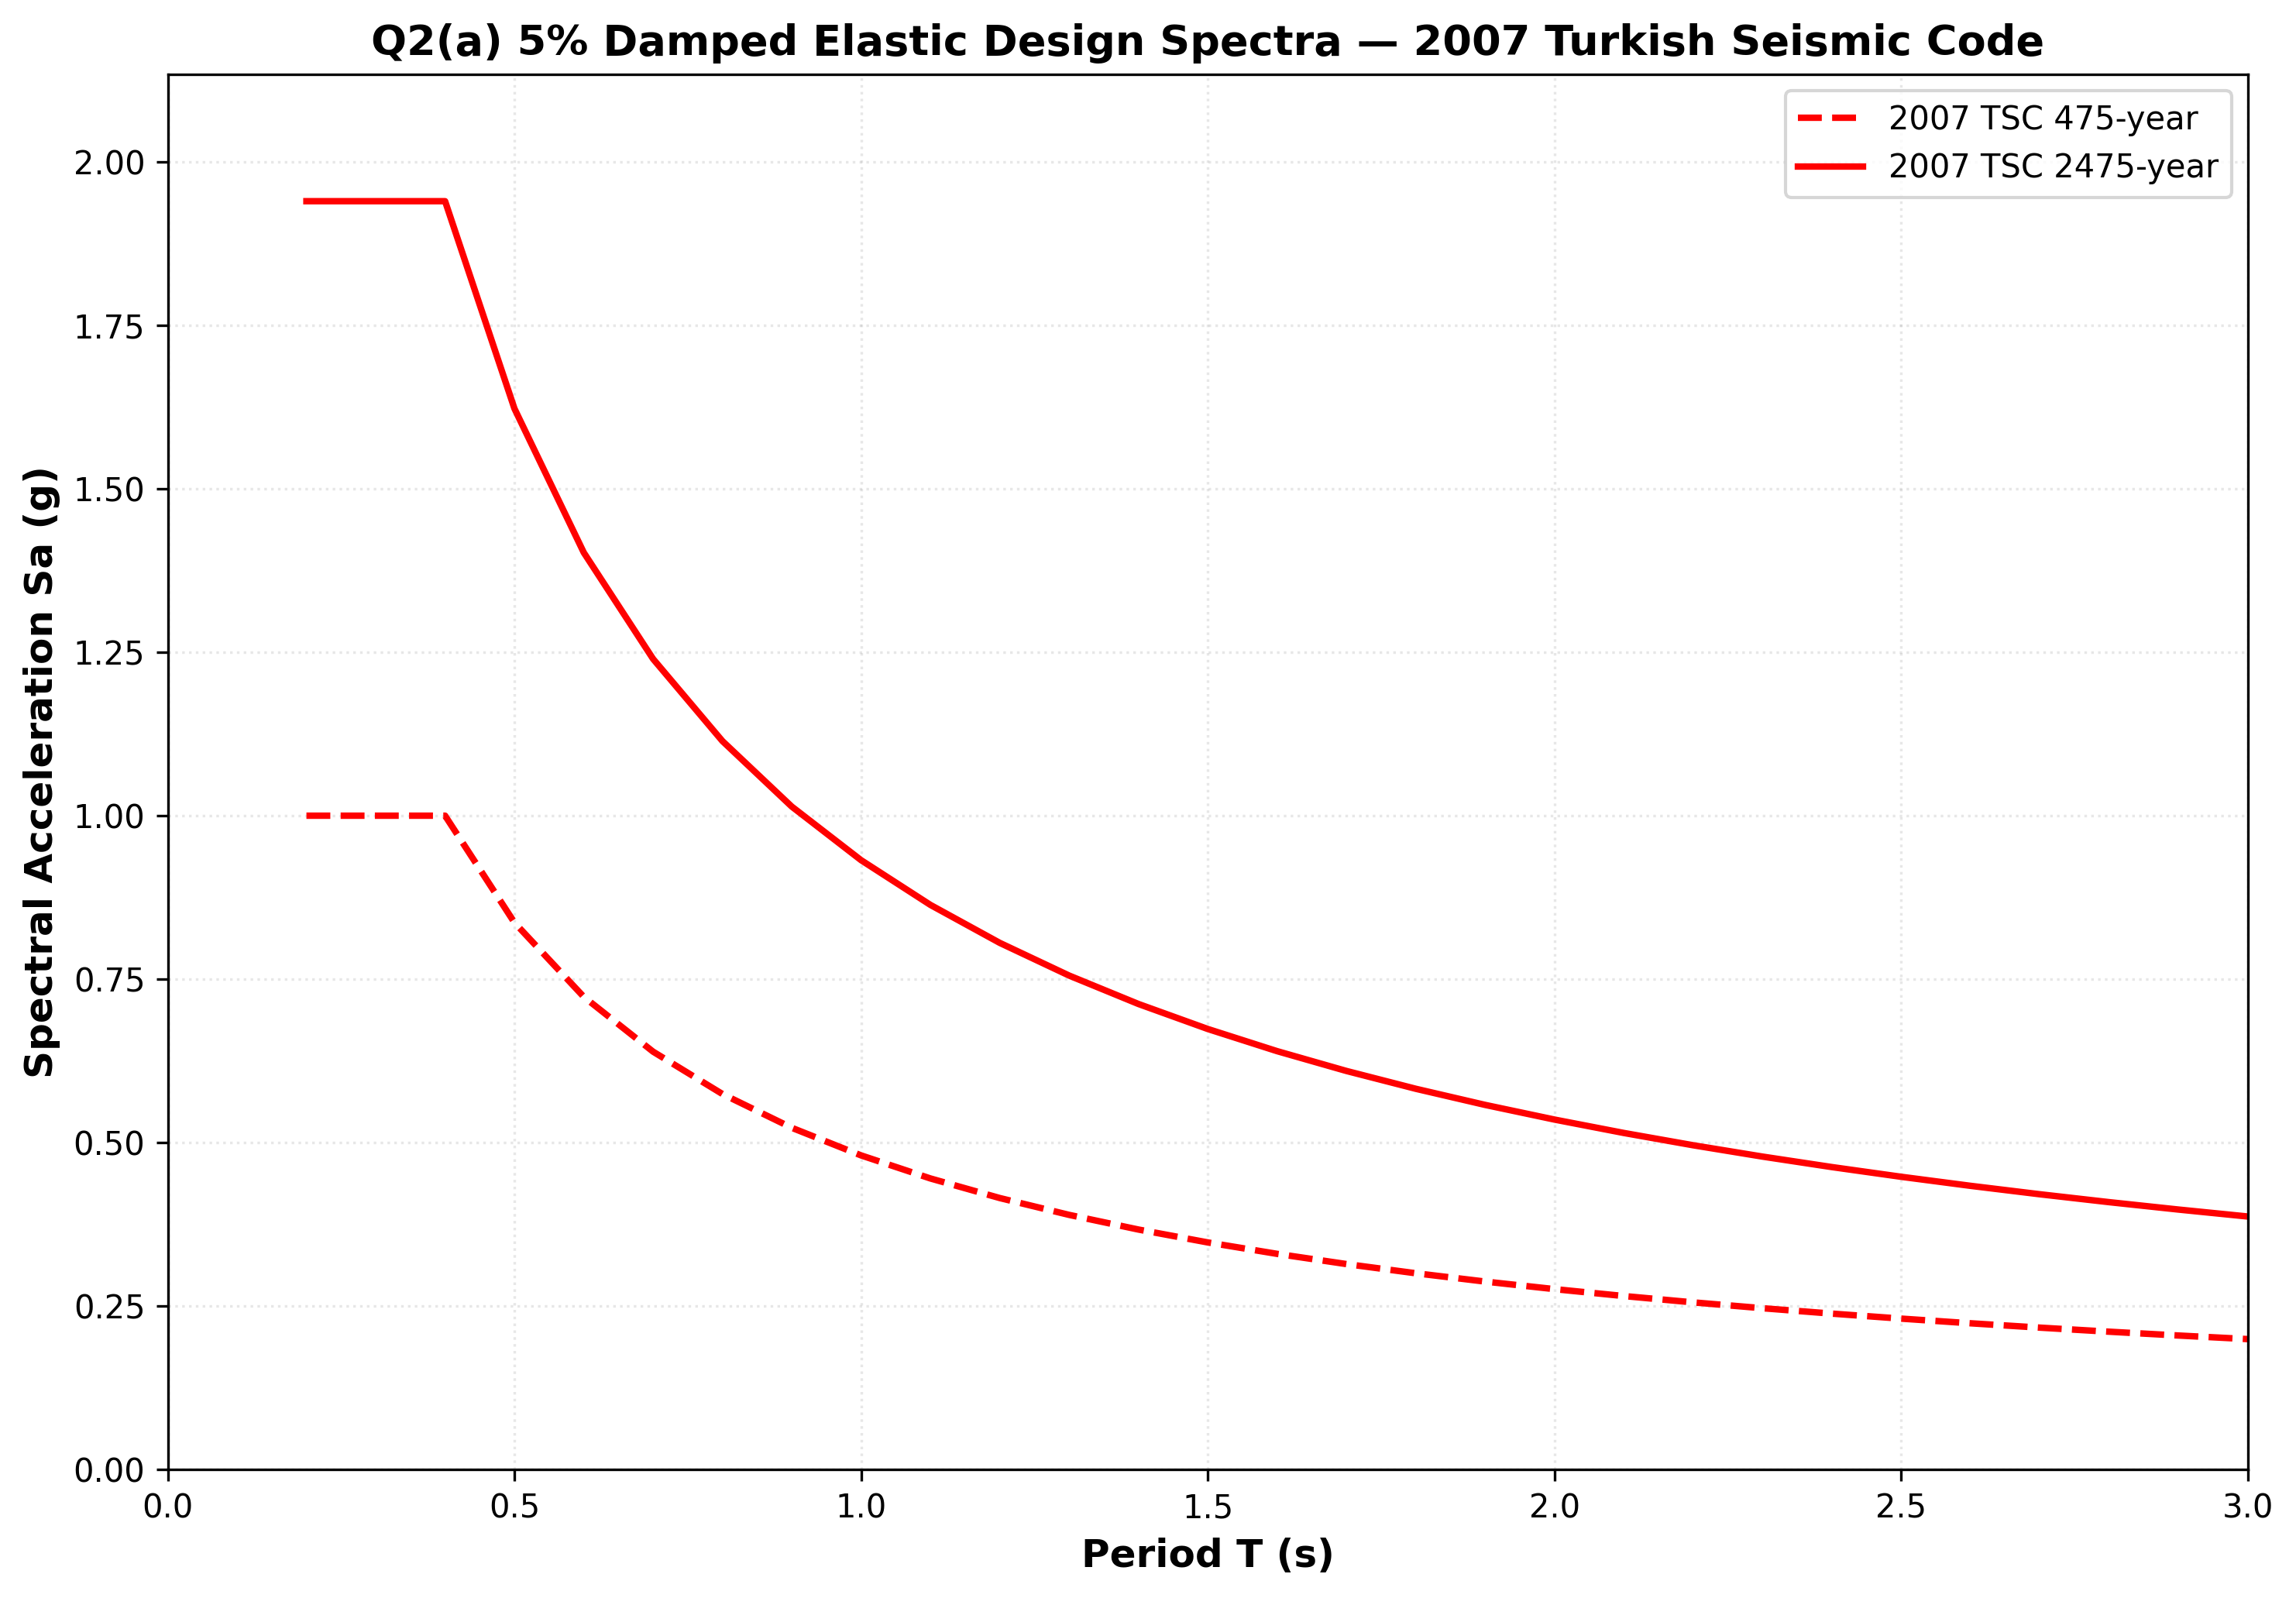
\includegraphics[width=0.95\textwidth]{results_q2/Q2a_2007_TSC_elastic_design_spectra.png}
    \caption{5\% damped elastic design spectra obtained using the 2007 Turkish Seismic Code.}
    \label{fig:q2a_2007}
\end{figure}

% ------------------------------------------------------------
\subsection{Q2(b): 2018 Turkish Building Earthquake Code Elastic Design Spectra}
% ------------------------------------------------------------

The 2018 Turkish Building Earthquake Code uses site-specific spectral parameters obtained from the Turkish Earthquake Hazard Map. For the assigned site, the official AFAD TDTH reports were obtained for DD-2 and DD-1 earthquake ground motion levels. DD-2 corresponds to the 475-year return period, while DD-1 corresponds to the 2475-year return period.

The TDTH parameters used in this study are summarized in Table~\ref{tab:tdth_values}.

\begin{table}[H]
\centering
\caption{AFAD TDTH spectral parameters for Dinar, ZC soil class.}
\label{tab:tdth_values}
\begin{tabular}{lccccccccc}
\toprule
Level & Return Period & $S_S$ & $S_1$ & $F_S$ & $F_1$ & $S_{DS}$ & $S_{D1}$ & PGA (g) & PGV (cm/s) \\
\midrule
DD-2 & 475 yr  & 0.608 & 0.147 & 1.257 & 1.500 & 0.764 & 0.220 & 0.256 & 13.680 \\
DD-1 & 2475 yr & 1.235 & 0.284 & 1.200 & 1.500 & 1.482 & 0.426 & 0.508 & 27.835 \\
\bottomrule
\end{tabular}
\end{table}

The 2018 horizontal elastic design spectrum is defined using $S_{DS}$ and $S_{D1}$. The corner periods are

\[
    T_A = 0.2\frac{S_{D1}}{S_{DS}}
\]

and

\[
    T_B = \frac{S_{D1}}{S_{DS}}
\]

with

\[
    T_L = 6.0\text{ s}
\]

For DD-2,

\[
    T_A = 0.2\frac{0.220}{0.764}=0.0576\text{ s}
\]

\[
    T_B = \frac{0.220}{0.764}=0.2880\text{ s}
\]

For DD-1,

\[
    T_A = 0.2\frac{0.426}{1.482}=0.0575\text{ s}
\]

\[
    T_B = \frac{0.426}{1.482}=0.2874\text{ s}
\]

These values are consistent with the periods reported by TDTH.

The 2018 horizontal elastic acceleration spectrum was calculated as

\[
S_{ae,2018}(T)=
\begin{cases}
S_{DS}\left(0.4+0.6\dfrac{T}{T_A}\right), & 0 \leq T \leq T_A \\[0.35cm]
S_{DS}, & T_A < T \leq T_B \\[0.35cm]
\dfrac{S_{D1}}{T}, & T_B < T \leq T_L \\[0.35cm]
\dfrac{S_{D1}T_L}{T^2}, & T_L < T
\end{cases}
\]

Figure~\ref{fig:q2b_2018} shows the 5\% damped elastic design spectra obtained using the 2018 Turkish Building Earthquake Code.

\begin{figure}[H]
    \centering
    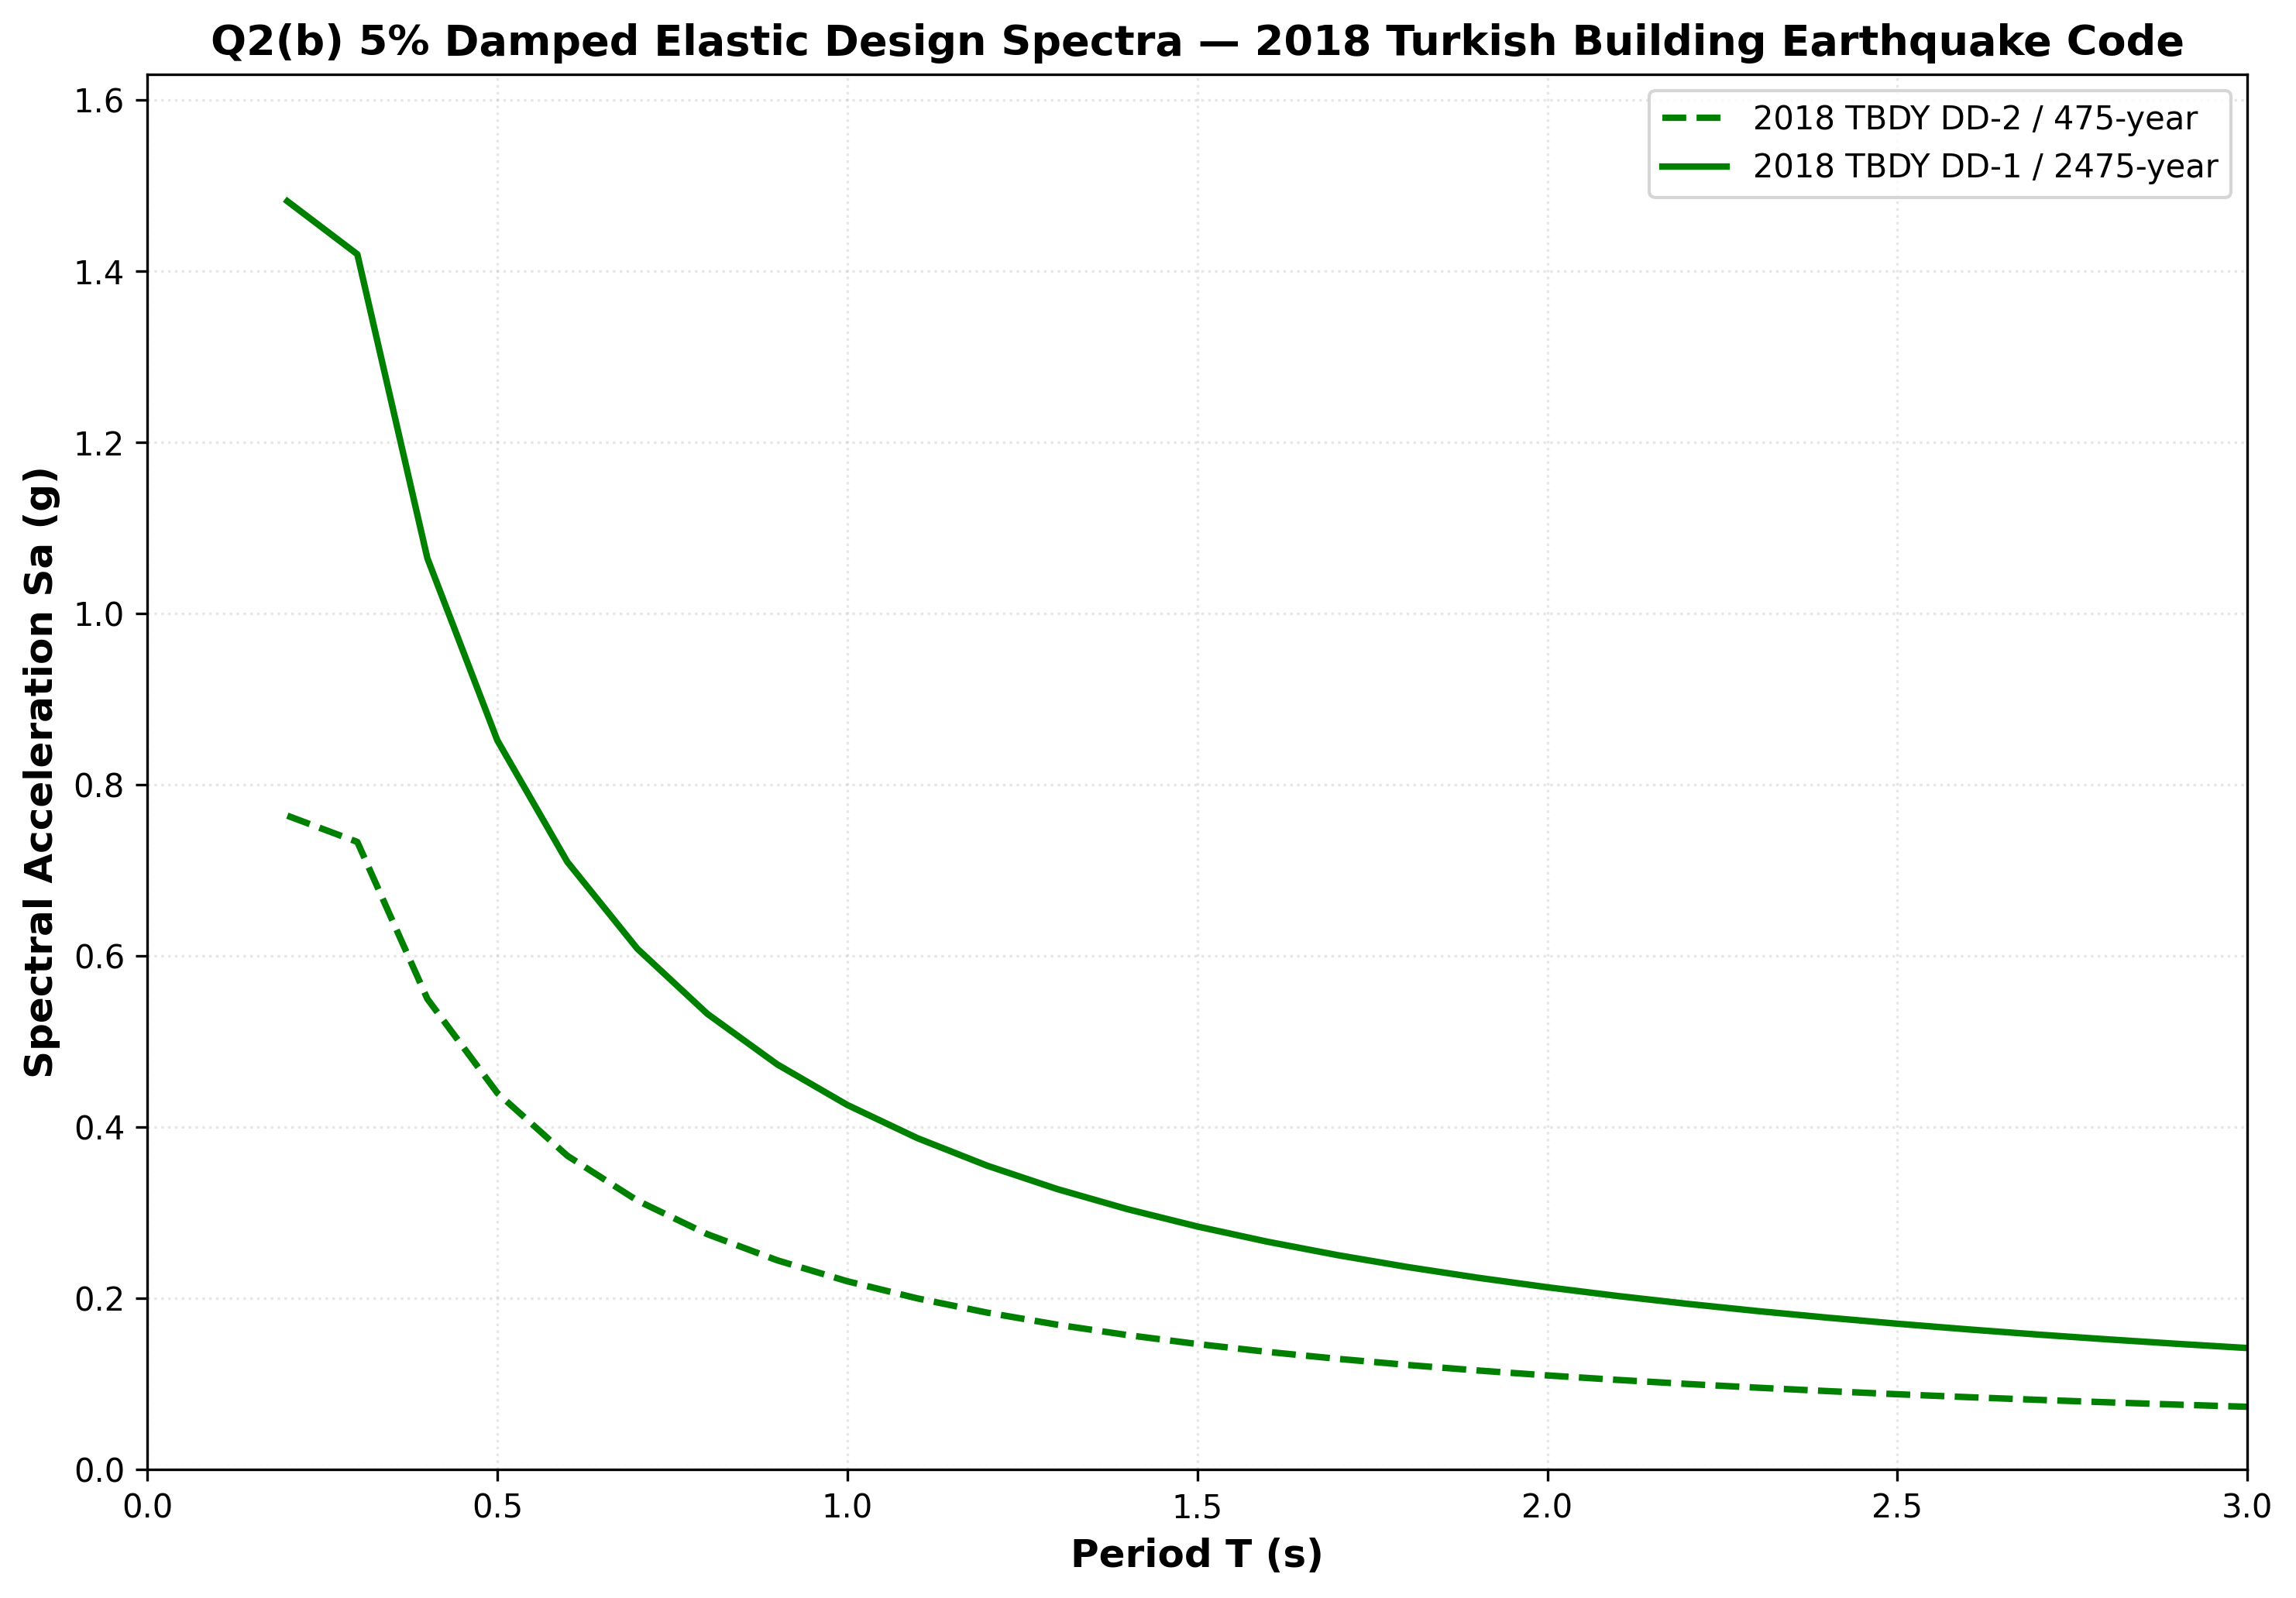
\includegraphics[width=0.95\textwidth]{results_q2/Q2b_2018_TBDY_elastic_design_spectra.png}
    \caption{5\% damped elastic design spectra obtained using the 2018 Turkish Building Earthquake Code.}
    \label{fig:q2b_2018}
\end{figure}

% ------------------------------------------------------------
\subsection{Q2(c): Comparison with the DIN95Y01 Elastic Response Spectrum}
% ------------------------------------------------------------

The 5\% damped acceleration response spectrum obtained from the DIN95Y01 ground motion record was compared with the elastic design spectra from the 2007 and 2018 Turkish seismic codes. The comparison is shown in Figure~\ref{fig:q2c_elastic_comparison}.

\begin{figure}[H]
    \centering
    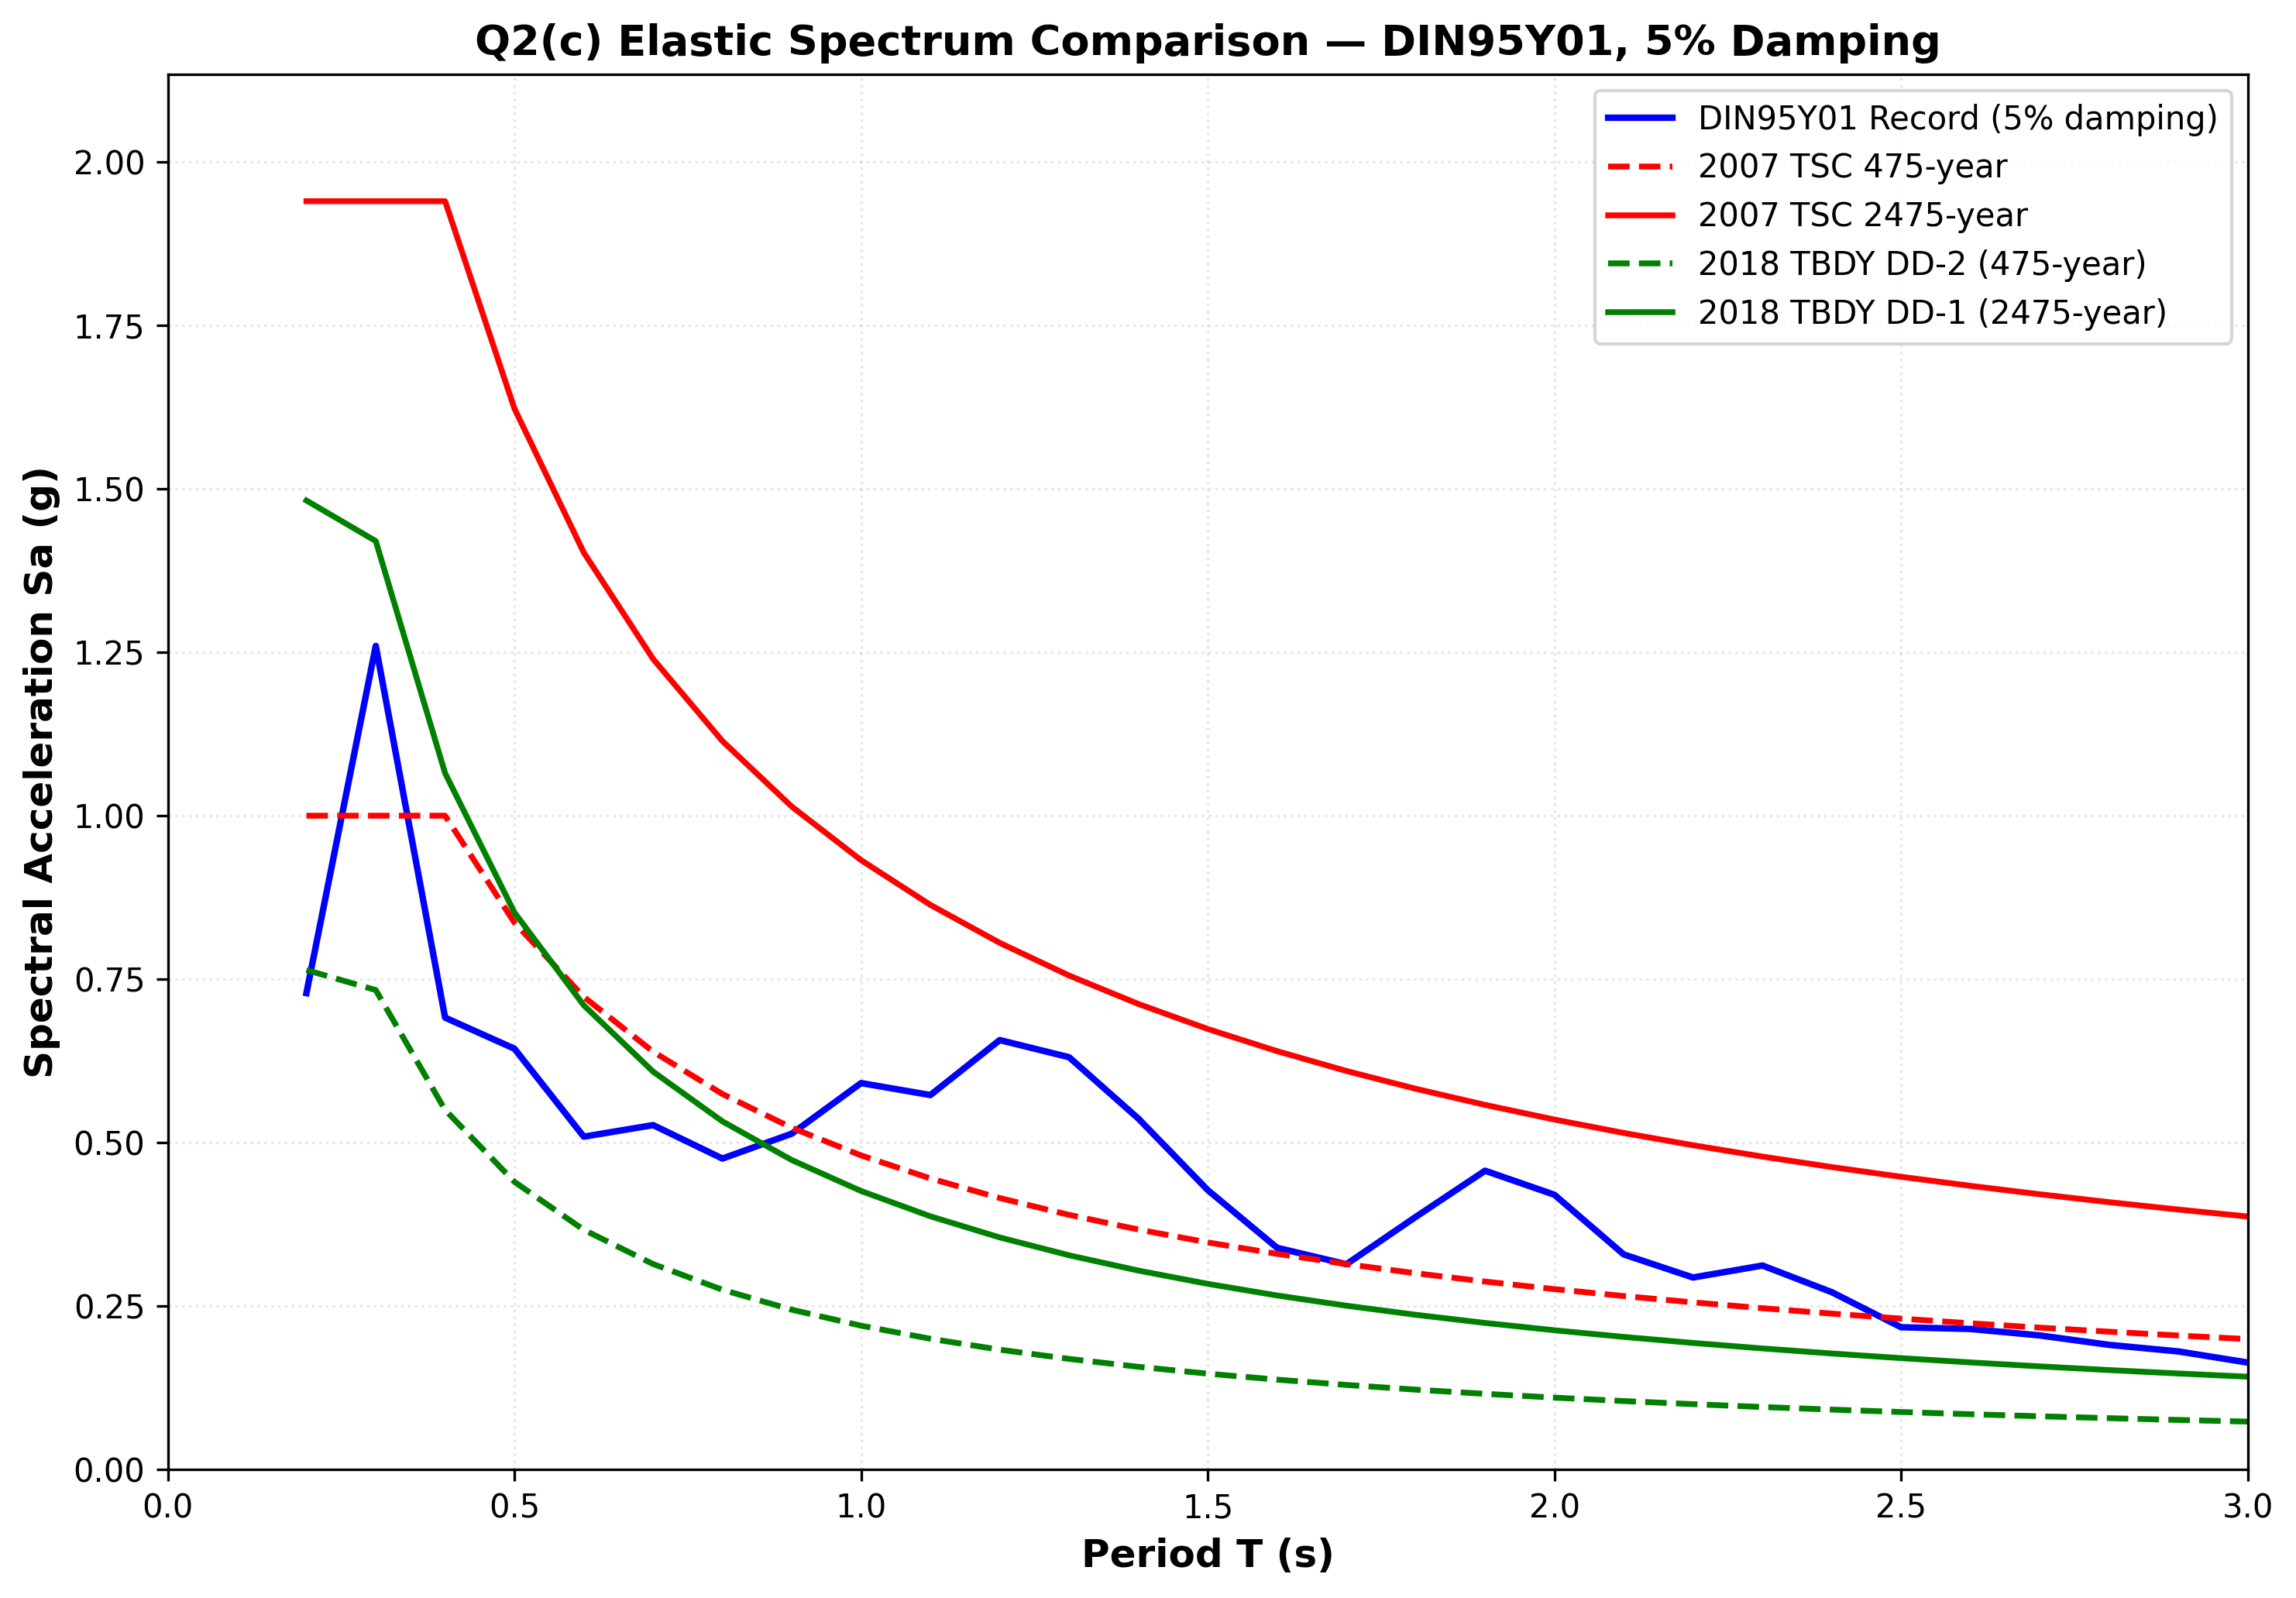
\includegraphics[width=0.95\textwidth]{results_q2/Q2c_elastic_comparison.png}
    \caption{Comparison of the DIN95Y01 5\% damped elastic acceleration spectrum with the 2007 and 2018 code-based elastic design spectra.}
    \label{fig:q2c_elastic_comparison}
\end{figure}

The 2475-year spectra are larger than the corresponding 475-year spectra for both the 2007 and 2018 code-based approaches, as expected. The 2018 spectra are site-specific because they are obtained from the AFAD TDTH parameters for the assigned coordinates and ZC soil class. In contrast, the 2007 spectra are based on seismic zone, importance factor, and local site class assumptions. Therefore, the 2018 spectrum provides a more location-specific representation of the seismic hazard.

The DIN95Y01 record spectrum is irregular because it is obtained from a single recorded accelerogram. It exceeds some of the 475-year design spectrum ordinates in selected period ranges, especially near the short-period peak and in parts of the intermediate-period range. However, it generally remains below the 2475-year spectra. This indicates that a single ground motion record does not necessarily envelope the code-based spectrum over the full period range.

% ------------------------------------------------------------
\subsection{Q2(d): Inelastic Spectra for Constant R-Factors}
% ------------------------------------------------------------

The assignment requires inelastic spectra to be obtained using constant response modification factors without performing nonlinear time-history analysis. Therefore, the inelastic spectra were calculated by dividing the corresponding elastic spectra by the selected $R$ value:

\[
    S_{a,R}(T)=\frac{S_{a,e}(T)}{R}
\]

Two values were considered:

\[
    R=4
\]

and

\[
    R=8
\]

This reduction was applied to the following spectra:

\begin{itemize}
    \item the record-based 5\% damped elastic acceleration spectrum,
    \item the 2007 TSC 475-year elastic spectrum,
    \item the 2007 TSC 2475-year elastic spectrum,
    \item the 2018 TBDY DD-2 elastic spectrum,
    \item the 2018 TBDY DD-1 elastic spectrum.
\end{itemize}

Figure~\ref{fig:q2d_r4} shows the inelastic spectra for $R=4$, while Figure~\ref{fig:q2d_r8} shows the corresponding spectra for $R=8$.

\begin{figure}[H]
    \centering
    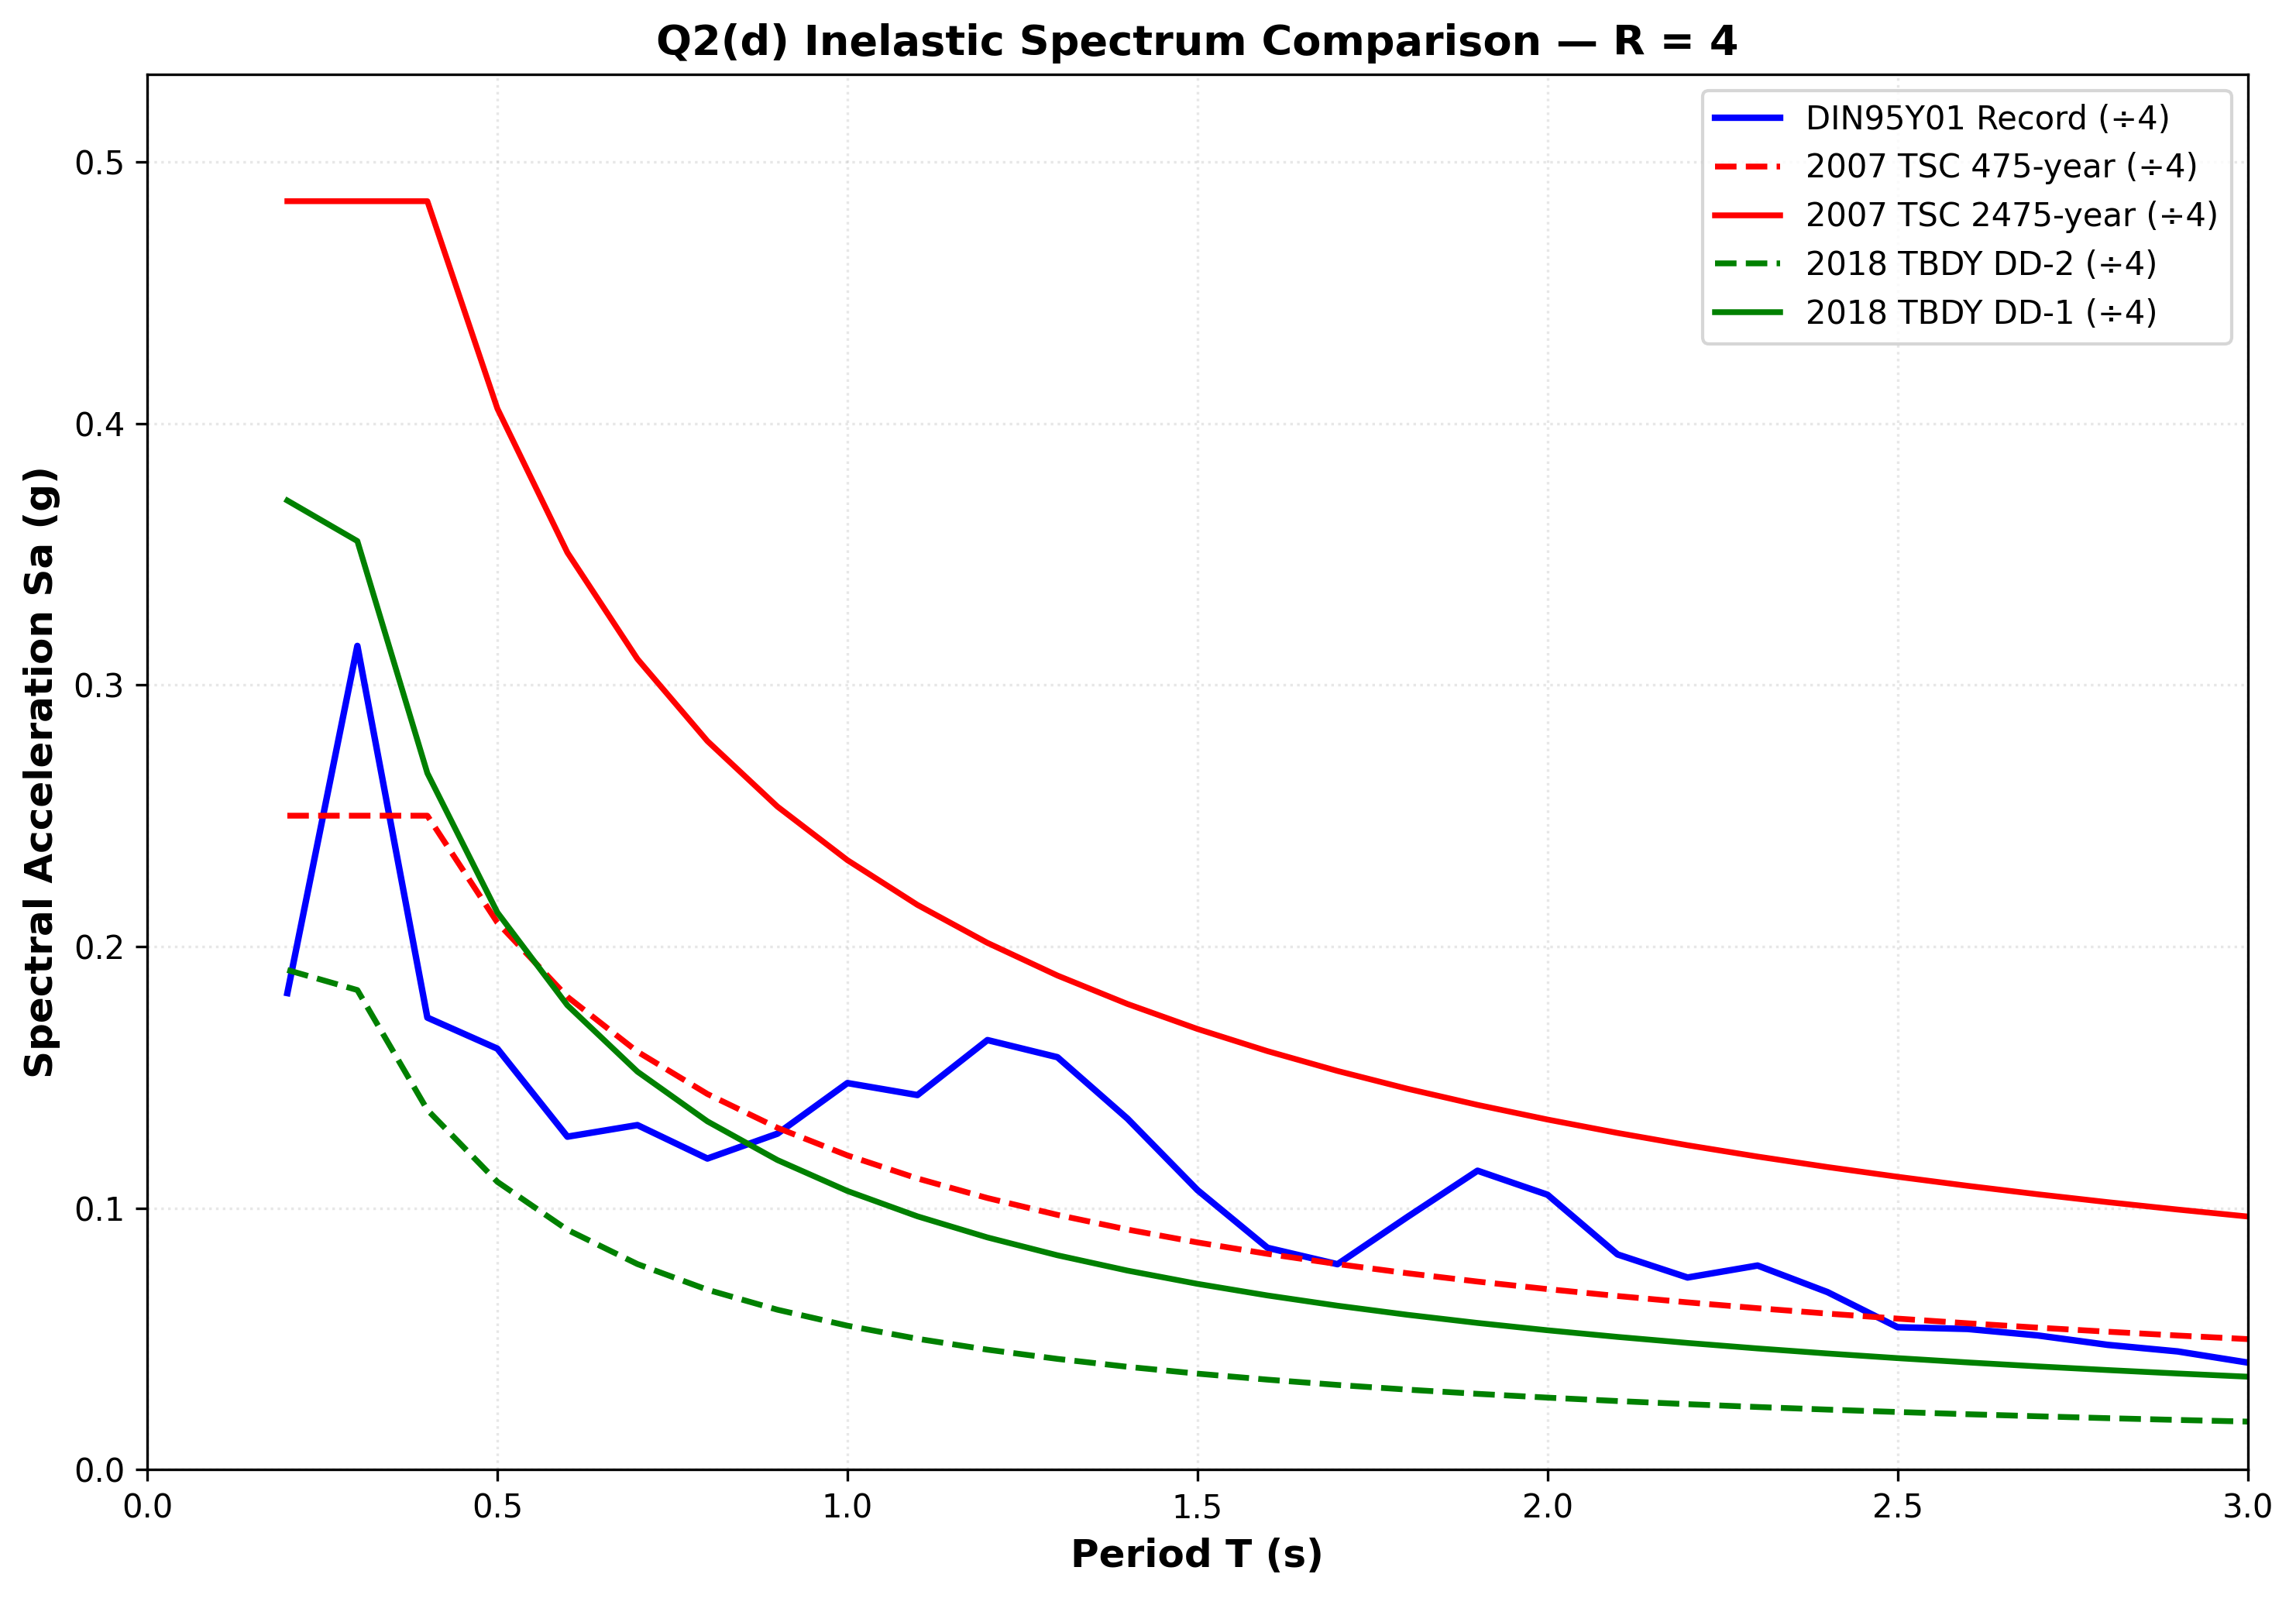
\includegraphics[width=0.95\textwidth]{results_q2/Q2d_inelastic_R4_comparison.png}
    \caption{Comparison of inelastic spectra for constant response modification factor $R=4$.}
    \label{fig:q2d_r4}
\end{figure}

\begin{figure}[H]
    \centering
    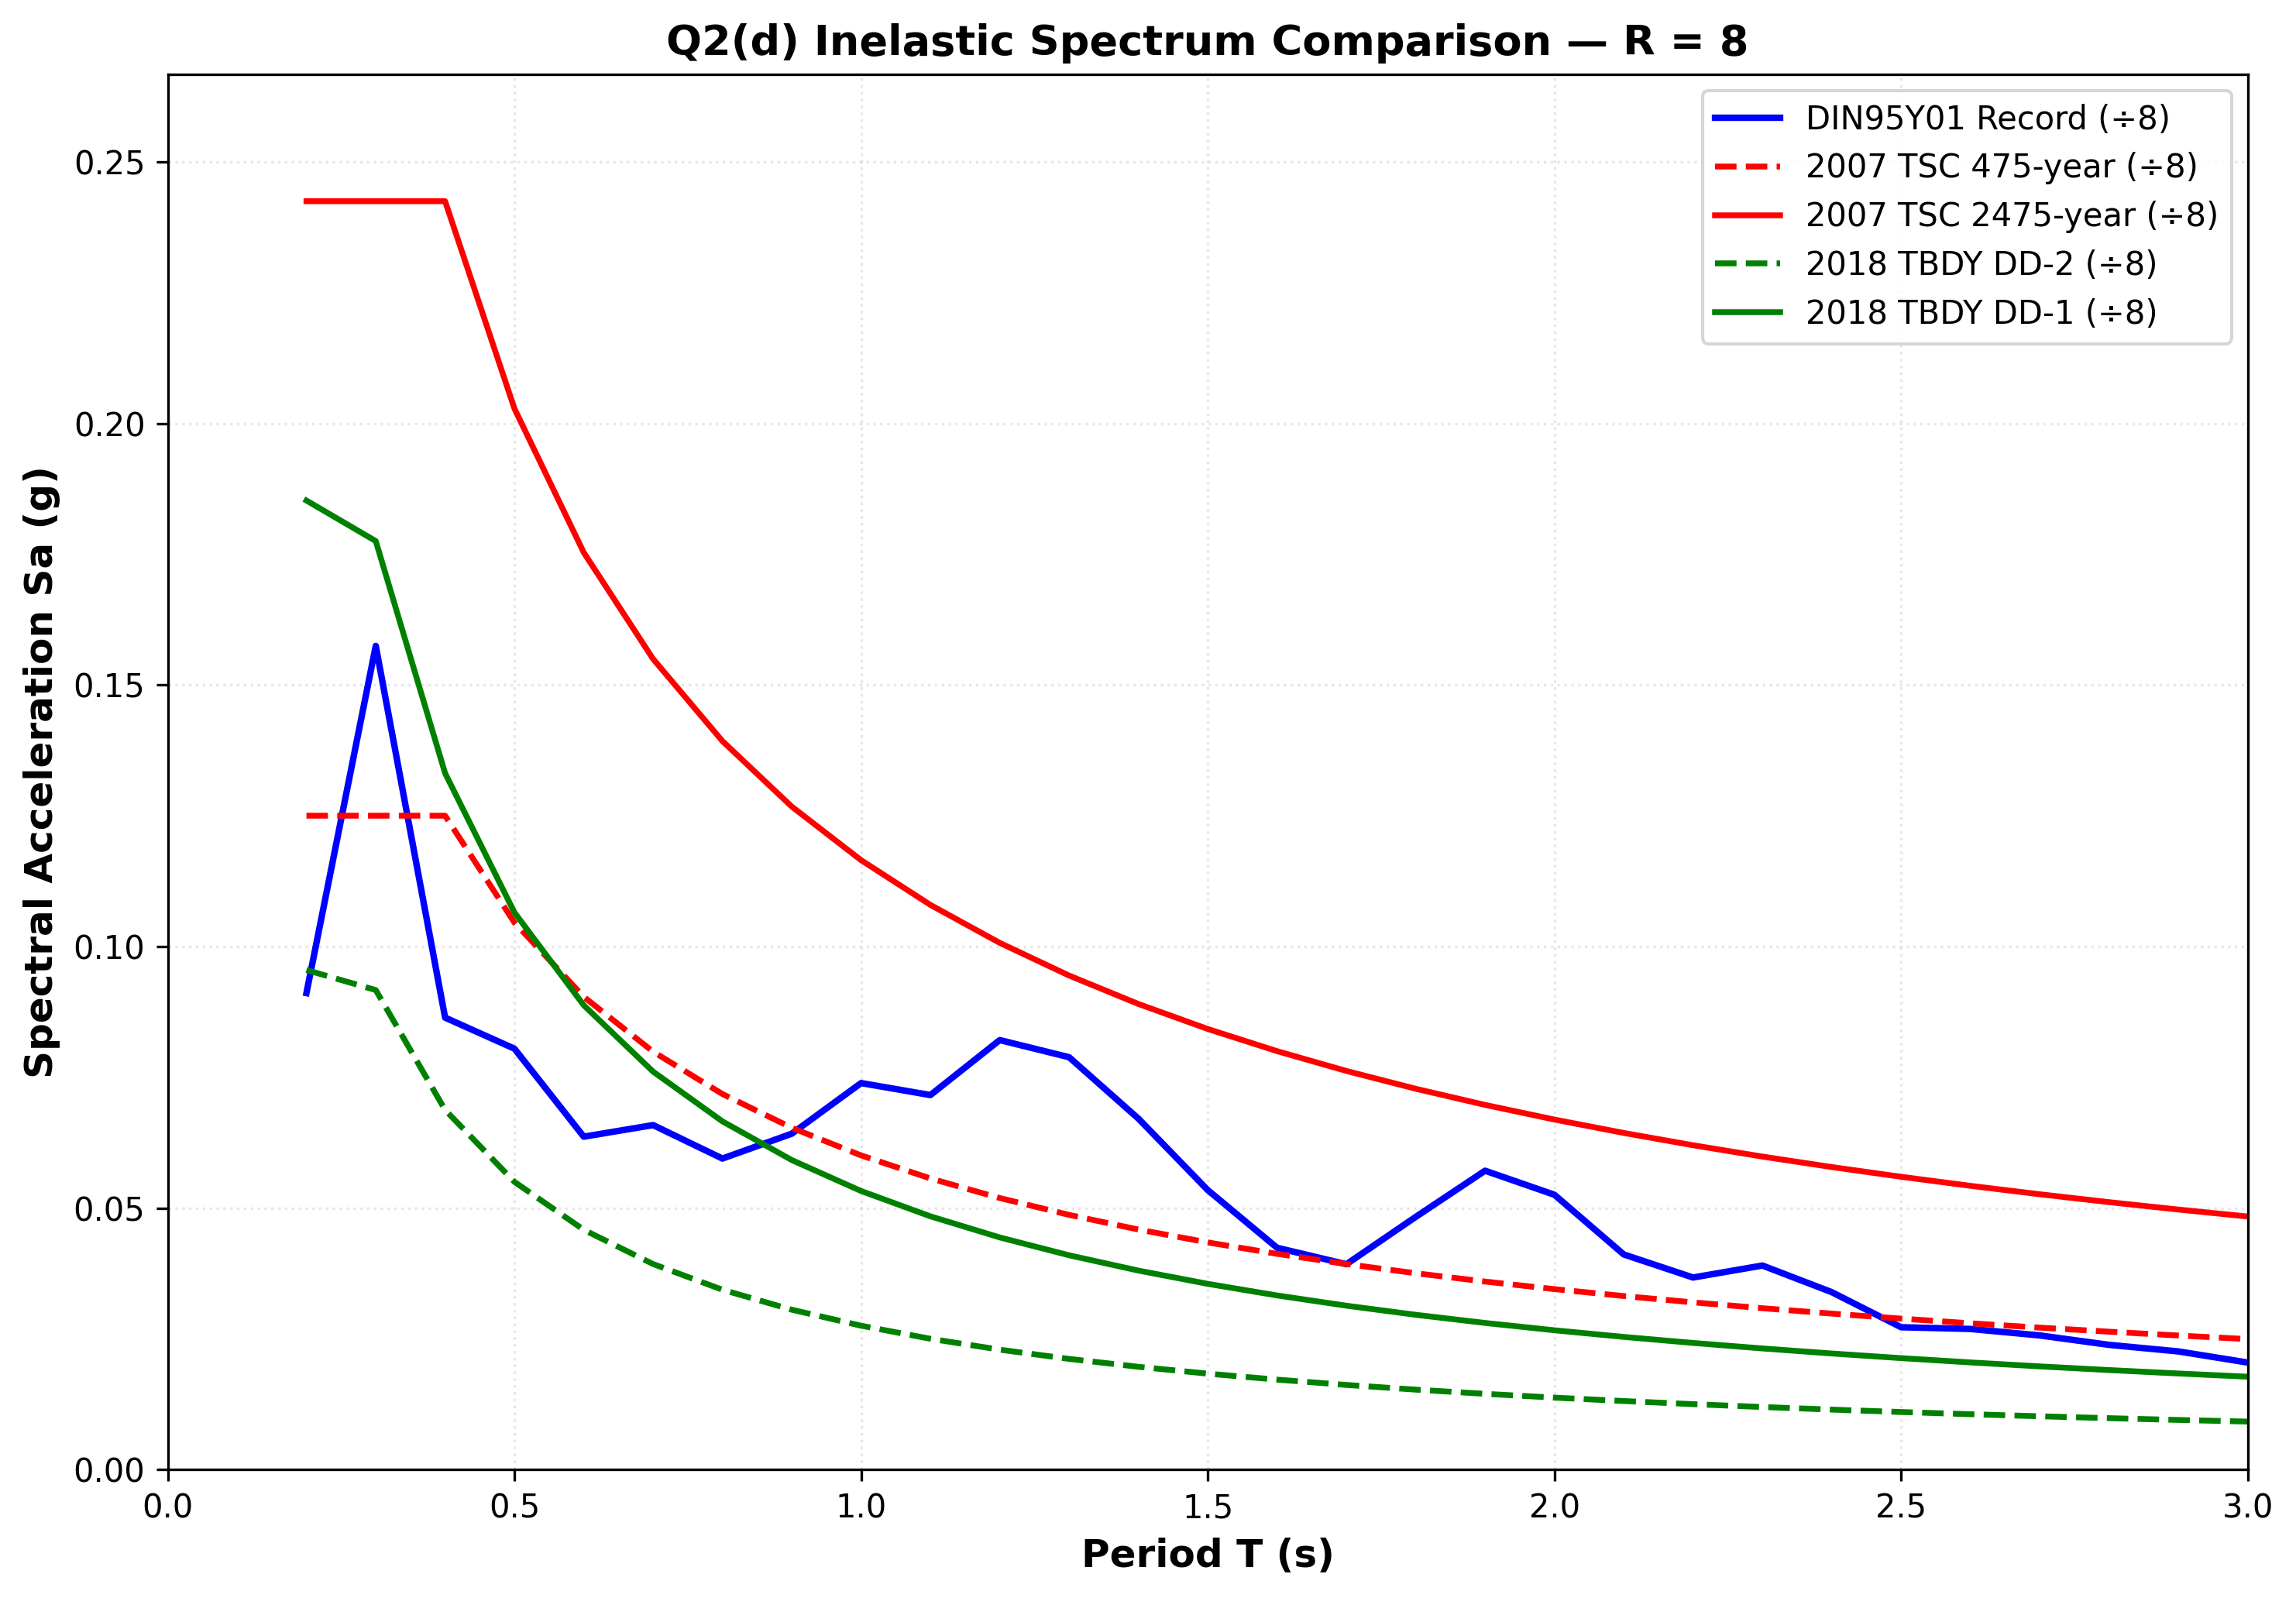
\includegraphics[width=0.95\textwidth]{results_q2/Q2d_inelastic_R8_comparison.png}
    \caption{Comparison of inelastic spectra for constant response modification factor $R=8$.}
    \label{fig:q2d_r8}
\end{figure}

The $R=8$ spectra have one-half of the corresponding $R=4$ ordinates because both were obtained using direct constant reduction of the elastic spectra. Increasing the response modification factor reduces the design spectral acceleration demand. However, this reduction implies greater reliance on ductility, energy dissipation, and acceptable inelastic deformation capacity of the structural system. Therefore, although larger $R$ values reduce design force demand, they require a structural system capable of sustaining larger inelastic deformation demands without brittle failure.

% ------------------------------------------------------------
\subsection{Q2 Discussion}
% ------------------------------------------------------------

The 2007 and 2018 Turkish seismic code spectra were obtained for the assigned Dinar site and compared with the DIN95Y01 5\% damped elastic acceleration response spectrum. The 2018 spectra were based on official TDTH parameters for DD-2 and DD-1 earthquake ground motion levels, while the 2007 spectra were obtained using code-based assumptions for seismic zone and local site class. The comparison shows that the 2475-year spectra produce higher spectral acceleration demands than the 475-year spectra. The record-based spectrum has local peaks that may exceed the design spectra at some periods, but it does not consistently envelope the code spectra over the full period range. Finally, inelastic spectra for $R=4$ and $R=8$ were obtained by constant reduction of the corresponding elastic spectra, showing the expected decrease in force demand with increasing response modification factor.

\section{Verification and Validation}

To ensure the correctness of the computed spectra, several consistency checks were performed:

\begin{enumerate}
    \item \textbf{Record Metadata Check:} The ground motion file was verified to contain 2796 points with a time step of 0.01 s and a total duration of 27.95 seconds. These parameters are consistent with the assignment specification.
    
    \item \textbf{PGA Check:} The peak ground acceleration was computed from the input acceleration array as 313.190 cm/s\(^2\), equivalent to 0.3194 g. This value represents a significant seismic input and is consistent with instrumental recordings from moderate earthquakes.
    
    \item \textbf{Damping Trend Check:} Across all periods, increasing the damping ratio from 2\% to 5\% to 10\% consistently results in a reduction in spectral ordinates, consistent with structural dynamics theory and energy dissipation principles.
    
    \item \textbf{Pseudo-Acceleration Formula Check:} A numerical verification was performed at a representative point in the response spectrum. At \(T = 2.0\) s and \(\xi = 5\%\), the displacement spectrum is approximately \(S_d \approx 0.415\) m. The corresponding natural frequency is:
    \begin{equation}
    \omega_n = \frac{2\pi}{2.0} = \pi \text{ rad/s}
    \end{equation}
    The pseudo-acceleration is then:
    \begin{equation}
    S_{a,\text{pseudo}} = \pi^2 \times 0.415 \approx 4.10 \text{ m/s}^2 \approx 0.418 g
    \end{equation}
    This value is consistent with the pseudo-acceleration plotted in Figure~\ref{fig:q1b_pseudo_acceleration} near \(T = 2.0\) s, confirming the correct implementation of the spectral formulas.
\end{enumerate}

The assignment specification permits the use of external verification software such as SeismoSignal or OpenSeesPy. The results presented in this report are based on the Newmark-beta integration code developed in Python, which has been verified through internal consistency checks as described above.

\section{Conclusion}

Elastic response spectra have been computed successfully for the DIN95Y01 ground motion record using the Newmark-beta constant average acceleration method. Key findings are as follows:

\begin{itemize}
    \item The strongest acceleration demand occurs in the short-period range, with a peak spectral acceleration of approximately 1.26 g at \(T \approx 0.3\) s for 5\% damping.
    
    \item Displacement demand becomes increasingly significant in the longer-period range (beyond 1 s), with maximum displacement reaching approximately 0.17 m for 5\% damping near \(T \approx 1.1\) s.
    
    \item Increasing the damping ratio from 2\% to 10\% consistently reduces spectral response across all periods, with reductions of approximately 40--50\% at most periods.
    
    \item The pseudo-acceleration and actual acceleration spectra are very close for this record, especially at the standard engineering damping of 5\%. This close agreement indicates that pseudo-acceleration is a suitable and accurate approximation for practical response-spectrum interpretation.
    
    \item The response spectra computed in this analysis provide the fundamental design input for elastic and inelastic spectral analysis of structures subjected to the DIN95Y01 earthquake record.
\end{itemize}

\section*{Appendix A: Python Code}

The full Python script \texttt{hw3\_response\_spectra.py} used to compute the response spectra presented in this report is submitted together with this document. The script contains detailed comments explaining the numerical implementation, the Newmark-beta integration scheme, and the computation of spectral quantities. The script is designed to be self-contained and can be executed independently to reproduce all results presented in this report.

\end{document}
